\documentclass[border=10pt]{standalone}

\usepackage{tikz}
\usepackage{tikzsymbols}
\usetikzlibrary{calc,patterns,shapes.geometric}

\def\centerarc[#1](#2)(#3:#4:#5){\draw[#1] ($(#2)+({#5*cos(#3)},{#5*sin(#3)})$) arc (#3:#4:#5);}

\begin{document}
	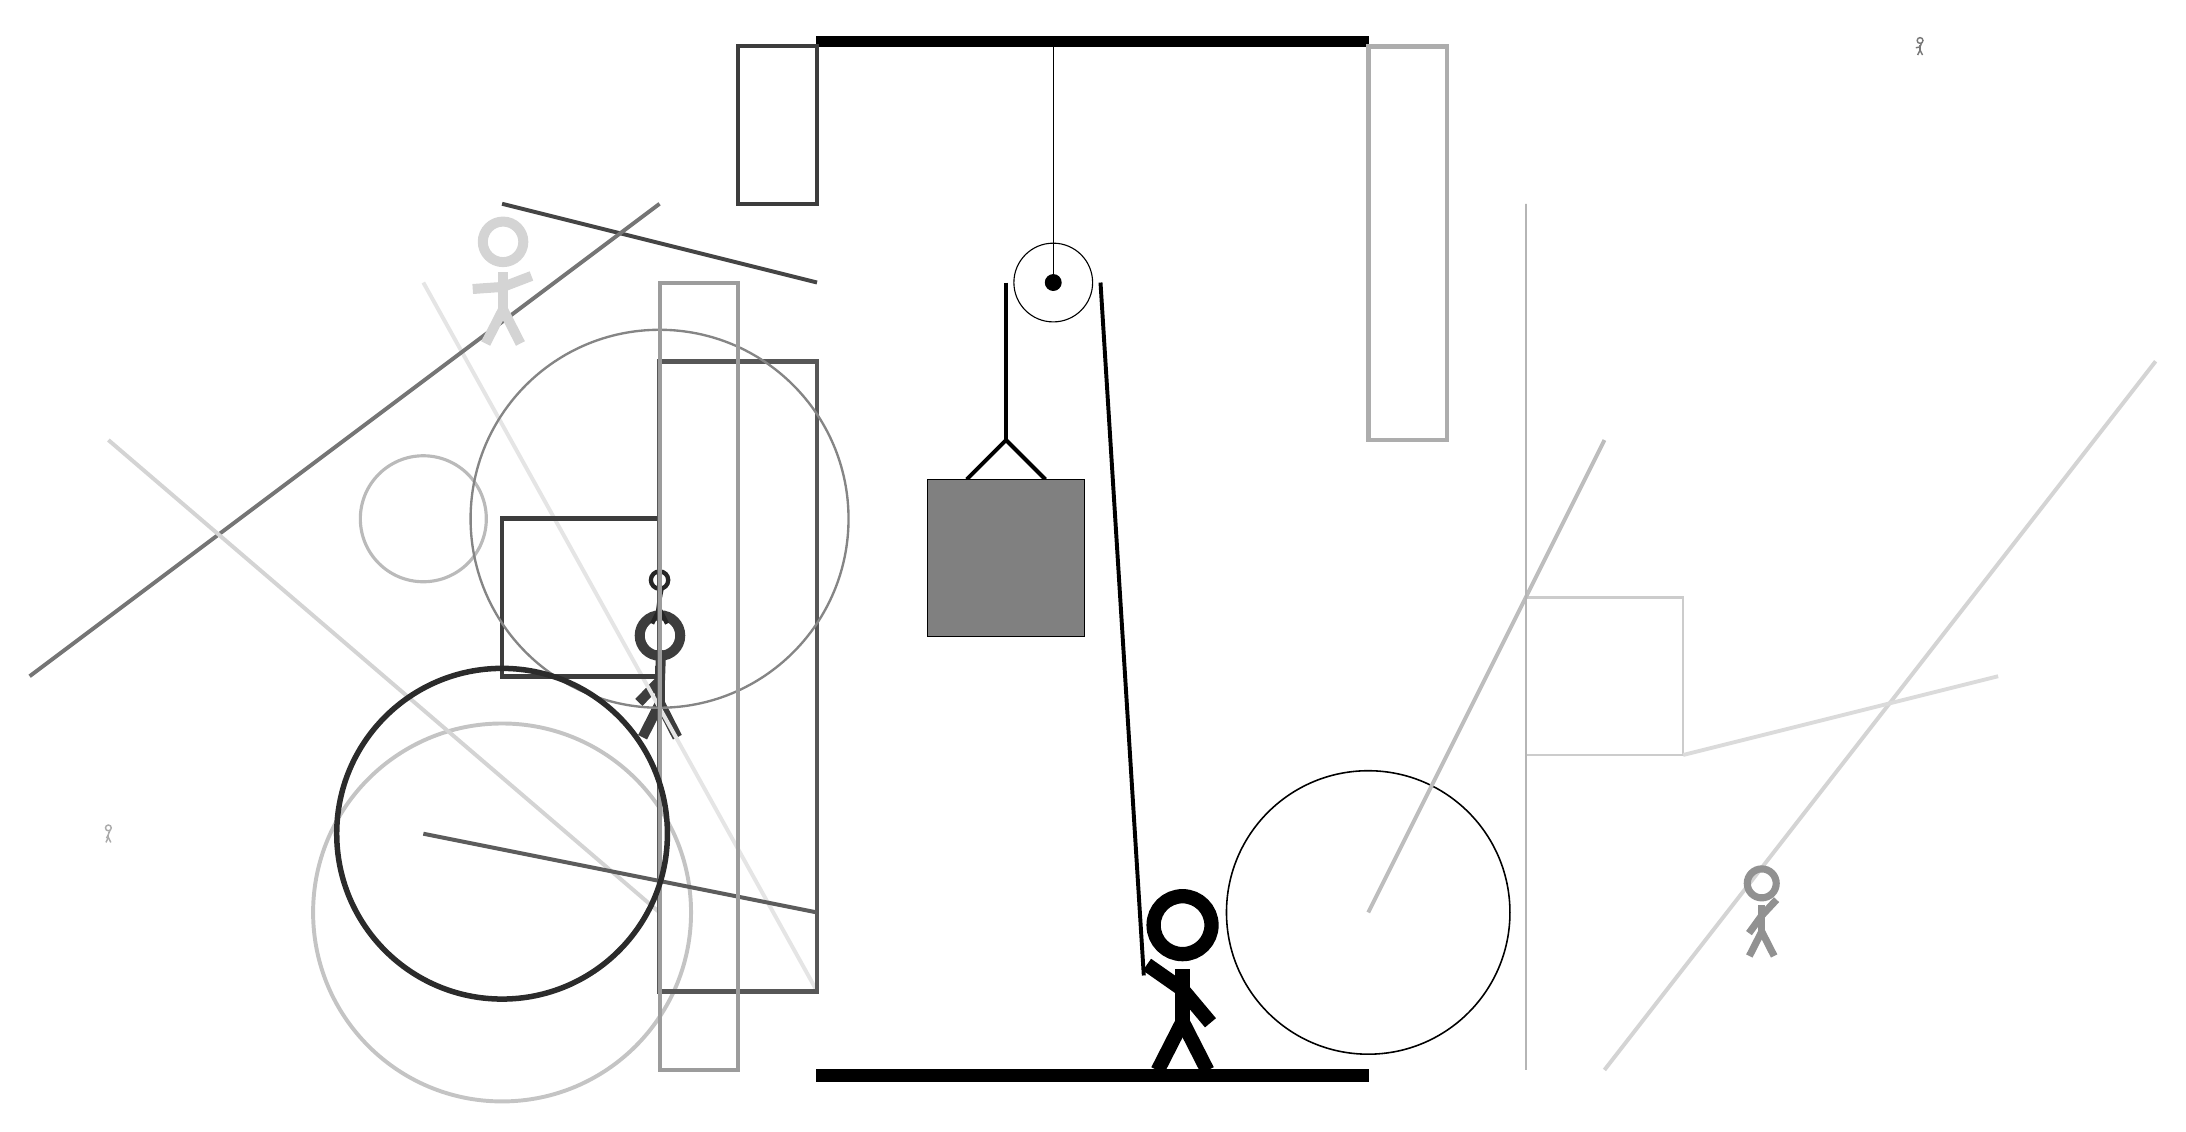
\begin{tikzpicture}
		%%%%% START %%%%%
		
		\draw[fill=black] (-2, 10) rectangle (5, 10.125);
		
		\draw (1, 7) circle (0.5);
		\draw[fill=black] (1, 7) circle (0.1);
		\draw (1, 10) -- (1, 7);
		
		\draw[line width=0.5mm] (-0.1, 4.5) -- (0.4, 5.0) -- (0.9, 4.5);
		\draw[fill=black!50] (-0.6, 4.5) rectangle (1.4, 2.5);
		
		\draw[line width=0.3mm, color=black!20] (7, 1) rectangle (9, 3);
		
		\draw [line width=0.5mm, color=black!23](-6, -1) circle (2.4);
		\node[line width=0.6mm, color=black!76] at (-4, 2) {\Strichmaxerl[7][46][88]};
		\draw[line width=0.5mm, color=black!10](-2, -2) -- (-7, 7);
		\draw[line width=0.5mm, color=black!17](8, -3) -- (15, 6);
		\node[line width=0.6mm, color=black!85] at (-4, 3) {\Strichmaxerl[3][83][79]};
		\draw [line width=0.2mm, color=black!100](5, -1) circle (1.8);
		\draw[line width=0.5mm, color=black!73](-6, 8) -- (-2, 7);
		\draw[line width=0.5mm, color=black!26](5, -1) -- (8, 5);
		\draw [line width=0.4mm, color=black!27](-7, 4) circle (0.8);
		\draw[line width=0.6mm, color=black!32] (5, 10) rectangle (6, 5);
		
		\draw[line width=0.5mm, color=black!54](-4, 8) -- (-12, 2);
		\node[line width=0.2mm, color=black!53] at (12, 10) {\Strichmaxerl[1][11][71]};
		\node[line width=0.6mm, color=black!43] at (10, -1) {\Strichmaxerl[5][54][47]};
		\draw[line width=0.3mm, color=black!29] (7, -3) rectangle (7, 8);
		\draw[line width=0.5mm, color=black!14](9, 1) -- (13, 2);
		\node[line width=0.3mm, color=black!33] at (-11, 0) {\Strichmaxerl[1][64][68]};
		\draw[line width=0.5mm, color=black!17](-4, -1) -- (-11, 5);
		\draw[line width=0.6mm, color=black!76] (-4, 4) rectangle (-6, 2);
		
		\draw[line width=0.6mm, color=black!66] (-4, 6) rectangle (-2, -2);
		\draw[line width=0.5mm, color=black!76] (-2, 8) rectangle (-3, 10);
		\draw[line width=0.5mm, color=black!64](-7, 0) -- (-2, -1);
		\draw [line width=0.3mm, color=black!48](-4, 4) circle (2.4);
		\draw[line width=0.5mm, color=black!39] (-4, 7) rectangle (-3, -3);
		\draw [line width=0.7mm, color=black!83](-6, 0) circle (2.1);
		
		\node[line width=0.4mm, color=black!17] at (-6, 7) {\Strichmaxerl[7][4][21]};
		
		
		\draw[line width=0.5mm] (0.4, 7) -- (0.4, 5.0);
		\centerarc[line width=0.5mm](1, 7)(0:180:0.6);
		\draw[line width=0.5mm](1.6, 7) -- (2.15, -1.8);
		
		\node at (2.6, -1.9) {\Strichmaxerl[10][-35][-50]};
		
		\draw[fill=black] (-2, -3) rectangle (5, -3.15);
		
		%%%%% END %%%%%
	\end{tikzpicture}
\end{document}